\subsection{OpenStack at the Edge}

Several open source communities have been formed to realize Edge computing use-cases using OpenStack. Most architectures use a Cloud and an Edge part that need to run synchronously to achieve the objectives. The key challenges in realizing openstack at the edge is that the components of openstack require large memory footprint along with the messaging and database infrastructure that runs as backbone for openstack services. This cannot be afforded when deploying at the Edge devices which have limited resources. The idea has been to optimize the openstack services to fit the requirements of the Edge device constraints. Few examples of open source effors in this area include Akraino, EdgeX Foundry, StarlingX and a few more. The figure~\ref{fig:figure13} shows the representation of openstack services at the centralized DC and the edge devices. Depending on the computational capability of the edge device, it can be hosted as Large, Medium or Small Edge \cite{osedge}.

\begin{figure}[h!]
    \centering
    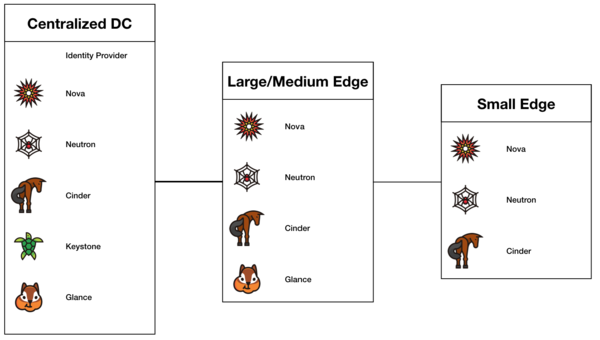
\includegraphics[width=0.9\textwidth]{openstack_edge}
    \label{fig:figure13}
    \caption{OpenStack Components for Edge Computing}
\end{figure}

The component services/daemons for each OpenStack can also be further customized based on the size of the Edge Device as illustrated in~\ref{fig:figure14} derived from \cite{osedge}.

\begin{figure}[h!]
    \centering
    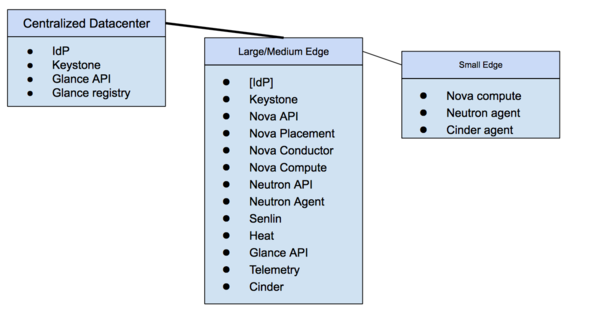
\includegraphics[width=0.9\textwidth]{openstack_edge_services}
    \label{fig:figure14}
    \caption{OpenStack Services for Edge Computing}
\end{figure}


